% Options for packages loaded elsewhere
\PassOptionsToPackage{unicode}{hyperref}
\PassOptionsToPackage{hyphens}{url}
%
\documentclass[
]{article}
\usepackage{amsmath,amssymb}
\usepackage{lmodern}
\usepackage{ifxetex,ifluatex}
\ifnum 0\ifxetex 1\fi\ifluatex 1\fi=0 % if pdftex
  \usepackage[T1]{fontenc}
  \usepackage[utf8]{inputenc}
  \usepackage{textcomp} % provide euro and other symbols
\else % if luatex or xetex
  \usepackage{unicode-math}
  \defaultfontfeatures{Scale=MatchLowercase}
  \defaultfontfeatures[\rmfamily]{Ligatures=TeX,Scale=1}
\fi
% Use upquote if available, for straight quotes in verbatim environments
\IfFileExists{upquote.sty}{\usepackage{upquote}}{}
\IfFileExists{microtype.sty}{% use microtype if available
  \usepackage[]{microtype}
  \UseMicrotypeSet[protrusion]{basicmath} % disable protrusion for tt fonts
}{}
\makeatletter
\@ifundefined{KOMAClassName}{% if non-KOMA class
  \IfFileExists{parskip.sty}{%
    \usepackage{parskip}
  }{% else
    \setlength{\parindent}{0pt}
    \setlength{\parskip}{6pt plus 2pt minus 1pt}}
}{% if KOMA class
  \KOMAoptions{parskip=half}}
\makeatother
\usepackage{xcolor}
\IfFileExists{xurl.sty}{\usepackage{xurl}}{} % add URL line breaks if available
\IfFileExists{bookmark.sty}{\usepackage{bookmark}}{\usepackage{hyperref}}
\hypersetup{
  pdftitle={5102 Data Analysis by Agency / Department},
  pdfauthor={CalEPA Racial Equity Workgroup},
  hidelinks,
  pdfcreator={LaTeX via pandoc}}
\urlstyle{same} % disable monospaced font for URLs
\usepackage[margin=1in]{geometry}
\usepackage{color}
\usepackage{fancyvrb}
\newcommand{\VerbBar}{|}
\newcommand{\VERB}{\Verb[commandchars=\\\{\}]}
\DefineVerbatimEnvironment{Highlighting}{Verbatim}{commandchars=\\\{\}}
% Add ',fontsize=\small' for more characters per line
\usepackage{framed}
\definecolor{shadecolor}{RGB}{248,248,248}
\newenvironment{Shaded}{\begin{snugshade}}{\end{snugshade}}
\newcommand{\AlertTok}[1]{\textcolor[rgb]{0.94,0.16,0.16}{#1}}
\newcommand{\AnnotationTok}[1]{\textcolor[rgb]{0.56,0.35,0.01}{\textbf{\textit{#1}}}}
\newcommand{\AttributeTok}[1]{\textcolor[rgb]{0.77,0.63,0.00}{#1}}
\newcommand{\BaseNTok}[1]{\textcolor[rgb]{0.00,0.00,0.81}{#1}}
\newcommand{\BuiltInTok}[1]{#1}
\newcommand{\CharTok}[1]{\textcolor[rgb]{0.31,0.60,0.02}{#1}}
\newcommand{\CommentTok}[1]{\textcolor[rgb]{0.56,0.35,0.01}{\textit{#1}}}
\newcommand{\CommentVarTok}[1]{\textcolor[rgb]{0.56,0.35,0.01}{\textbf{\textit{#1}}}}
\newcommand{\ConstantTok}[1]{\textcolor[rgb]{0.00,0.00,0.00}{#1}}
\newcommand{\ControlFlowTok}[1]{\textcolor[rgb]{0.13,0.29,0.53}{\textbf{#1}}}
\newcommand{\DataTypeTok}[1]{\textcolor[rgb]{0.13,0.29,0.53}{#1}}
\newcommand{\DecValTok}[1]{\textcolor[rgb]{0.00,0.00,0.81}{#1}}
\newcommand{\DocumentationTok}[1]{\textcolor[rgb]{0.56,0.35,0.01}{\textbf{\textit{#1}}}}
\newcommand{\ErrorTok}[1]{\textcolor[rgb]{0.64,0.00,0.00}{\textbf{#1}}}
\newcommand{\ExtensionTok}[1]{#1}
\newcommand{\FloatTok}[1]{\textcolor[rgb]{0.00,0.00,0.81}{#1}}
\newcommand{\FunctionTok}[1]{\textcolor[rgb]{0.00,0.00,0.00}{#1}}
\newcommand{\ImportTok}[1]{#1}
\newcommand{\InformationTok}[1]{\textcolor[rgb]{0.56,0.35,0.01}{\textbf{\textit{#1}}}}
\newcommand{\KeywordTok}[1]{\textcolor[rgb]{0.13,0.29,0.53}{\textbf{#1}}}
\newcommand{\NormalTok}[1]{#1}
\newcommand{\OperatorTok}[1]{\textcolor[rgb]{0.81,0.36,0.00}{\textbf{#1}}}
\newcommand{\OtherTok}[1]{\textcolor[rgb]{0.56,0.35,0.01}{#1}}
\newcommand{\PreprocessorTok}[1]{\textcolor[rgb]{0.56,0.35,0.01}{\textit{#1}}}
\newcommand{\RegionMarkerTok}[1]{#1}
\newcommand{\SpecialCharTok}[1]{\textcolor[rgb]{0.00,0.00,0.00}{#1}}
\newcommand{\SpecialStringTok}[1]{\textcolor[rgb]{0.31,0.60,0.02}{#1}}
\newcommand{\StringTok}[1]{\textcolor[rgb]{0.31,0.60,0.02}{#1}}
\newcommand{\VariableTok}[1]{\textcolor[rgb]{0.00,0.00,0.00}{#1}}
\newcommand{\VerbatimStringTok}[1]{\textcolor[rgb]{0.31,0.60,0.02}{#1}}
\newcommand{\WarningTok}[1]{\textcolor[rgb]{0.56,0.35,0.01}{\textbf{\textit{#1}}}}
\usepackage{graphicx}
\makeatletter
\def\maxwidth{\ifdim\Gin@nat@width>\linewidth\linewidth\else\Gin@nat@width\fi}
\def\maxheight{\ifdim\Gin@nat@height>\textheight\textheight\else\Gin@nat@height\fi}
\makeatother
% Scale images if necessary, so that they will not overflow the page
% margins by default, and it is still possible to overwrite the defaults
% using explicit options in \includegraphics[width, height, ...]{}
\setkeys{Gin}{width=\maxwidth,height=\maxheight,keepaspectratio}
% Set default figure placement to htbp
\makeatletter
\def\fps@figure{htbp}
\makeatother
\setlength{\emergencystretch}{3em} % prevent overfull lines
\providecommand{\tightlist}{%
  \setlength{\itemsep}{0pt}\setlength{\parskip}{0pt}}
\setcounter{secnumdepth}{-\maxdimen} % remove section numbering
\usepackage{booktabs}
\usepackage{longtable}
\usepackage{array}
\usepackage{multirow}
\usepackage{wrapfig}
\usepackage{float}
\usepackage{colortbl}
\usepackage{pdflscape}
\usepackage{tabu}
\usepackage{threeparttable}
\usepackage{threeparttablex}
\usepackage[normalem]{ulem}
\usepackage{makecell}
\usepackage{xcolor}
\ifluatex
  \usepackage{selnolig}  % disable illegal ligatures
\fi

\title{5102 Data Analysis by Agency / Department}
\author{CalEPA Racial Equity Workgroup}
\date{\emph{Updated: 2021-06-14}}

\begin{document}
\maketitle

{
\setcounter{tocdepth}{5}
\tableofcontents
}
\hypertarget{data-analysis-by-agency-department}{%
\section{5102 Data Analysis by Agency /
Department}\label{data-analysis-by-agency-department}}

\hypertarget{introduction}{%
\subsection{Introduction}\label{introduction}}

intro text\ldots{}

\hypertarget{resources}{%
\subsection{Resources}\label{resources}}

\hypertarget{census-data}{%
\subsubsection{Census Data:}\label{census-data}}

\begin{itemize}
\item
  tidycensus R package:
  \url{https://walker-data.com/tidycensus/articles/basic-usage.html}
\item
  general census workshop w/ R:
  \url{https://jennhuck.github.io/workshops/tidycensus.html}
\item
  ACS Table B02001 data (race w/o hispanic/latino data):
  \url{https://censusreporter.org/data/table/?table=B02001\&geo_ids=04000US06}
\item
  ACS Table B03002 data (race with hispanic/latino data):
  \url{https://censusreporter.org/data/table/?table=B03002\&geo_ids=04000US06}
\item
  info about race in census data:
  \url{https://censusreporter.org/topics/race-hispanic/}
\item
  other general info about concepts and tables in census data:
  \url{https://censusreporter.org/topics/}
\item
  check/validation of the numbers for CA:
  \url{https://www.ppic.org/publication/californias-population/}
\end{itemize}

\hypertarget{ca-workforce-data}{%
\subsubsection{CA Workforce Data:}\label{ca-workforce-data}}

\begin{itemize}
\item
  CalHR data page:
  \url{https://www.calhr.ca.gov/pages/statewide-reports.aspx}
\item
  Workforce data on CA open data portal:
  \url{https://data.ca.gov/dataset/calhr-civil-rights-data-for-gare-capital-cohort-2019}
\end{itemize}

\hypertarget{enter-parameters}{%
\subsection{Enter Parameters}\label{enter-parameters}}

Enter the year of the most recently published 5102 report and the most
recently published ACS data, and if needed edit the URL for the 5102
data set on the California Open Data Portal. Also, edit default plot
titles and captions as needed (CalEPA and its 6 Boards, Departments, and
Offices {[}BDOs{]} are the examples used here).

\begin{Shaded}
\begin{Highlighting}[]
\CommentTok{\# enter parameters (for current reporting year) {-}{-}{-}{-}{-}{-}{-}{-}{-}{-}{-}{-}{-}{-}{-}{-}{-}{-}{-}{-}{-}{-}{-}{-}{-}{-}{-}{-}{-}}
\NormalTok{report\_year }\OtherTok{\textless{}{-}} \DecValTok{2020}
\NormalTok{acs\_data\_year }\OtherTok{\textless{}{-}} \DecValTok{2019}

\NormalTok{agency\_name }\OtherTok{\textless{}{-}} \StringTok{\textquotesingle{}CalEPA\textquotesingle{}}

\NormalTok{url\_data\_all\_yrs }\OtherTok{\textless{}{-}} \StringTok{\textquotesingle{}https://data.ca.gov/dataset/e620a64f{-}6b86{-}4ce0{-}ab4b{-}03d06674287b/resource/aba87ad9{-}f6b0{-}4a7e{-}a45e{-}d1452417eb7f/download/calhr\_5102\_statewide\_2011{-}2020.csv\textquotesingle{}}

\NormalTok{default\_pl\_title }\OtherTok{\textless{}{-}} \FunctionTok{glue}\NormalTok{(}\StringTok{\textquotesingle{}\{agency\_name\} Workforce Compared to State Population (Year \{report\_year\})\textquotesingle{}}\NormalTok{)}
\NormalTok{default\_pl\_title\_groups }\OtherTok{\textless{}{-}} \FunctionTok{glue}\NormalTok{(}\StringTok{\textquotesingle{}\{agency\_name\} Workforce by Occupation and Ethnicity Group Compared to State Population (Year \{report\_year\})\textquotesingle{}}\NormalTok{)}
\NormalTok{default\_pl\_title\_bdo }\OtherTok{\textless{}{-}} \FunctionTok{glue}\NormalTok{(}\StringTok{\textquotesingle{}\{agency\_name\} Workforce by BDO Compared to State Population (Year \{report\_year\})\textquotesingle{}}\NormalTok{)}

\NormalTok{default\_pl\_subtitle }\OtherTok{\textless{}{-}} \FunctionTok{element\_blank}\NormalTok{()}
\NormalTok{default\_pl\_caption }\OtherTok{\textless{}{-}} \FunctionTok{glue}\NormalTok{(}\StringTok{\textquotesingle{}Data sources: state population data from \{acs\_data\_year\} 1 yr American Community Survey  |  workforce data from \{report\_year\} CalHR 5102 Report\textquotesingle{}}\NormalTok{)}
\end{Highlighting}
\end{Shaded}

\hypertarget{load-transform-data}{%
\subsection{Load \& Transform Data}\label{load-transform-data}}

\hypertarget{data}{%
\subsubsection{5102 Data}\label{data}}

Info about 5102 dataset?\ldots{} from Key performance target document \&
notes accompanying slide deck\ldots.

\hypertarget{ethnicity-groupings}{%
\paragraph{Ethnicity Groupings}\label{ethnicity-groupings}}

describe ethnicity levels added to the 5102 dataset (level 1: BIPOC /
white, level 2: combined Asian and Pacific Islander groupings)\ldots{}

\begin{Shaded}
\begin{Highlighting}[]
\CommentTok{\# 1 {-} load / transform data {-}{-}{-}{-}{-}{-}{-}{-}{-}{-}{-}{-}{-}{-}{-}{-}{-}{-}{-}{-}{-}{-}{-}{-}{-}{-}{-}{-}{-}{-}{-}{-}{-}{-}{-}{-}{-}{-}{-}{-}{-}{-}{-}{-}{-}{-}{-}{-}{-}{-}{-}{-}{-}{-}{-}{-}{-}{-}{-}{-}{-}{-}{-}}

\DocumentationTok{\#\# 5102 {-}{-}{-}{-}}
\NormalTok{df\_5102 }\OtherTok{\textless{}{-}} \FunctionTok{read\_csv}\NormalTok{(url\_data\_all\_yrs) }\SpecialCharTok{\%\textgreater{}\%}
    \FunctionTok{clean\_names}\NormalTok{() }
\end{Highlighting}
\end{Shaded}

\begin{verbatim}
## 
## -- Column specification --------------------------------------------------------
## cols(
##   `As Of Date` = col_date(format = ""),
##   Dept = col_character(),
##   `Employee Category` = col_character(),
##   `Sub Category` = col_character(),
##   `SOC Code` = col_character(),
##   `Scheme Code` = col_character(),
##   `Class Code` = col_character(),
##   `Class Title` = col_character(),
##   `Identity Variable` = col_character(),
##   Gender = col_character(),
##   `Record Count` = col_double()
## )
\end{verbatim}

\begin{Shaded}
\begin{Highlighting}[]
\CommentTok{\# add additional levels for ethnicity grouping}
\CommentTok{\#   identity\_variable (in original dataset) is most detailed level}
\CommentTok{\#   level 1 groups all BIPOC together (resulting groups are BIPOC and white)}
\CommentTok{\#   level 2 groups some identity\_variable sub{-}groupings together (Asian group and Pacific Islander group)}
\NormalTok{df\_5102 }\OtherTok{\textless{}{-}}\NormalTok{ df\_5102 }\SpecialCharTok{\%\textgreater{}\%} 
    \FunctionTok{mutate}\NormalTok{(}
        \AttributeTok{ethnicity\_level1 =} \FunctionTok{case\_when}\NormalTok{(}
\NormalTok{            identity\_variable }\SpecialCharTok{==} \StringTok{\textquotesingle{}White\textquotesingle{}} \SpecialCharTok{\textasciitilde{}} \StringTok{\textquotesingle{}White\textquotesingle{}}\NormalTok{, }
            \ConstantTok{TRUE} \SpecialCharTok{\textasciitilde{}} \StringTok{\textquotesingle{}BIPOC\textquotesingle{}}\NormalTok{),}
        \AttributeTok{ethnicity\_level2 =} \FunctionTok{case\_when}\NormalTok{(}
            \FunctionTok{str\_detect}\NormalTok{(identity\_variable, }\StringTok{\textquotesingle{}Pacific Islander\textquotesingle{}}\NormalTok{) }\SpecialCharTok{\textasciitilde{}} \StringTok{\textquotesingle{}Pacific Islander\textquotesingle{}}\NormalTok{, }\CommentTok{\# groups (all start with "Pacific Islander {-} "): Guamanian, Hawaiian, Other or Multiple, and Samoan}
            \FunctionTok{str\_detect}\NormalTok{(identity\_variable, }\StringTok{\textquotesingle{}Asian\textquotesingle{}}\NormalTok{) }\SpecialCharTok{\textasciitilde{}} \StringTok{\textquotesingle{}Asian\textquotesingle{}}\NormalTok{, }\CommentTok{\# groups (all start with "Asian {-} "): Cambodian, Chinese, Filipino, Indian, Japanese, Korean, Laotian, Other or Multiple, Vietnamese}
            \ConstantTok{TRUE} \SpecialCharTok{\textasciitilde{}}\NormalTok{ identity\_variable)}
\NormalTok{    )}

\CommentTok{\# add a year column}
\NormalTok{df\_5102 }\OtherTok{\textless{}{-}}\NormalTok{ df\_5102 }\SpecialCharTok{\%\textgreater{}\%} 
    \FunctionTok{mutate}\NormalTok{(}\AttributeTok{reporting\_year =} \FunctionTok{year}\NormalTok{(as\_of\_date))}
\end{Highlighting}
\end{Shaded}

\hypertarget{filter-for-selected-agency}{%
\paragraph{Filter for Selected
Agency}\label{filter-for-selected-agency}}

Search for the name of your selected agency from the box below, then
copy and paste into the subsequent code chunk. List of agency names in
the 5102 dataset:

\begin{Shaded}
\begin{Highlighting}[]
\CommentTok{\# list of all departments}
\NormalTok{depts\_list }\OtherTok{\textless{}{-}}\NormalTok{ df\_5102 }\SpecialCharTok{\%\textgreater{}\%} 
    \FunctionTok{distinct}\NormalTok{(dept) }\SpecialCharTok{\%\textgreater{}\%} 
    \FunctionTok{arrange}\NormalTok{(dept) }\SpecialCharTok{\%\textgreater{}\%} 
    \FunctionTok{rename}\NormalTok{(}\StringTok{\textquotesingle{}Department Name\textquotesingle{}} \OtherTok{=}\NormalTok{ dept)}


\NormalTok{depts\_list }\SpecialCharTok{\%\textgreater{}\%} 
    \FunctionTok{kbl}\NormalTok{() }\SpecialCharTok{\%\textgreater{}\%} 
    \FunctionTok{kable\_paper}\NormalTok{() }\SpecialCharTok{\%\textgreater{}\%}
    \FunctionTok{scroll\_box}\NormalTok{(}\AttributeTok{width =} \StringTok{"500px"}\NormalTok{, }\AttributeTok{height =} \StringTok{"200px"}\NormalTok{) }\SpecialCharTok{\%\textgreater{}\%}
\NormalTok{    \{.\}}
\end{Highlighting}
\end{Shaded}

\begin{table}
\centering
\begin{tabular}[t]{l}
\hline
Department Name\\
\hline
Achieving a Better Life Experience for People With Disabilities, California\\
\hline
Administrative Law, Office of\\
\hline
African-American Museum, California\\
\hline
Aging, Commission on\\
\hline
Aging, Department of\\
\hline
Agricultural Association, 22nd District\\
\hline
Agricultural Association, 32nd District\\
\hline
Agricultural Associations\\
\hline
Agricultural Labor Relations Board\\
\hline
Air Resources Board\\
\hline
Alcohol and Drug Programs, Department of\\
\hline
Alcoholic Beverage Control Appeals Board\\
\hline
Alcoholic Beverage Control, Department of\\
\hline
Alternative Energy and Advanced Transportation Financing Authority\\
\hline
Arts Council, California\\
\hline
Baldwin Hills Conservancy\\
\hline
Business and Economic Development, Governor's Office of\\
\hline
Business Oversight, Department of\\
\hline
Business, Consumer Services, and Housing Agency\\
\hline
Business, Transportation, and Housing Agency\\
\hline
CA Complete Count, Census 2020\\
\hline
Child Support Services, Department of\\
\hline
Children and Families First Commission\\
\hline
Chiropractic Examiners, Board of\\
\hline
Coachella Valley Mountains Conservancy\\
\hline
Coastal Commission, California\\
\hline
Coastal Conservancy, State\\
\hline
Colorado River Board\\
\hline
Community Colleges, California\\
\hline
Community Services and Development, Department of\\
\hline
Compensation Insurance Fund, State\\
\hline
Conservation Corps, California\\
\hline
Conservation, Department of\\
\hline
Consumer Affairs, Department of\\
\hline
Controller, Office of the California State\\
\hline
Corrections and Rehabilitation, California Department of\\
\hline
Debt and Investment Advisory Commission, California\\
\hline
Debt Limit Allocation Committee, California\\
\hline
Delta Protection Commission\\
\hline
Delta Stewardship Council\\
\hline
Developmental Disabilities, State Council on\\
\hline
Developmental Services, Department of\\
\hline
Disability Access, California Commission on\\
\hline
Earthquake Authority, California\\
\hline
Education Audit Appeals Panel\\
\hline
Education, Department of\\
\hline
Educational Facilities Authority, California\\
\hline
Emergency Medical Services Authority\\
\hline
Emergency Services, California Governor's Office of\\
\hline
Employment Development Department\\
\hline
Employment Training Panel, California\\
\hline
Energy Resources Conservation and Development Commission\\
\hline
Environmental Health Hazard Assessment, Office of\\
\hline
Environmental Protection Agency\\
\hline
Equalization, Board of\\
\hline
Exposition and State Fair, California\\
\hline
Fair Employment and Housing Commission\\
\hline
Fair Employment and Housing, Department of\\
\hline
Fair Political Practices Commission\\
\hline
Finance, Department of\\
\hline
Financial Institutions, Department of\\
\hline
Financial Protection and Innovation, Department of\\
\hline
FISCal\\
\hline
Fish and Wildlife, Department of\\
\hline
Food and Agriculture, Department of\\
\hline
Forestry and Fire Protection, Department of\\
\hline
Franchise Tax Board\\
\hline
Gambling Control Commission, California\\
\hline
General Services, Department of\\
\hline
Government Operations Agency\\
\hline
Health and Human Services Agency\\
\hline
Health Benefit Exchange, California\\
\hline
Health Care Services, Department of\\
\hline
Health Facilities Financing Authority, California\\
\hline
Health Planning and Development, Office of Statewide\\
\hline
High Speed Rail Authority, California\\
\hline
Highway Patrol, California\\
\hline
Horse Racing Board, California\\
\hline
Housing and Community Development, Department of\\
\hline
Housing Finance Agency, California\\
\hline
Human Resources, California Department of\\
\hline
Independent Living Council, State\\
\hline
Industrial Relations, Department of\\
\hline
Inspector General, Office of the\\
\hline
Insurance, Department of\\
\hline
Justice, Department of\\
\hline
Labor and Workforce Development Agency\\
\hline
Law Revision Commission, California\\
\hline
Legislative Counsel, Office of\\
\hline
Library, California State\\
\hline
Little Hoover Commission\\
\hline
Lottery, California State\\
\hline
Managed Health Care, Department of\\
\hline
Managed Risk Medical Insurance Board\\
\hline
Mental Health Services Oversight and Accountability Commission\\
\hline
Military Department\\
\hline
Motor Vehicles, Department of\\
\hline
Native American Heritage Commission\\
\hline
Natural Resources Agency, California\\
\hline
Osteopathic Medical Board of California\\
\hline
Parks and Recreation, Department of\\
\hline
Peace Officer Standards and Training, Commission on\\
\hline
Personnel Board, State\\
\hline
Pesticide Regulation, Department of\\
\hline
Pilot Commissioners, Board of\\
\hline
Pollution Control Financing Authority, California\\
\hline
Postsecondary Education Commission, California\\
\hline
Prison Industry Authority, California\\
\hline
Public Defender, Office of the State\\
\hline
Public Employees' Retirement System, California\\
\hline
Public Employment Relations Board\\
\hline
Public Health, California Department of\\
\hline
Public Utilities Commission, California\\
\hline
Real Estate Appraisers, Office of\\
\hline
Real Estate, Department of\\
\hline
Rehabilitation, Department of\\
\hline
Resources Recycling and Recovery, Department of\\
\hline
Sacramento-San Joaquin Delta Conservancy\\
\hline
San Diego River Conservancy\\
\hline
San Francisco Bay Conservation and Development Commission\\
\hline
San Gabriel Lower Los Angeles Rivers and Mountains Conservancy\\
\hline
San Joaquin River Conservancy\\
\hline
Santa Monica Mountains Conservancy\\
\hline
Scholarshare Investment Board\\
\hline
School Finance Authority, California\\
\hline
Science Center, California\\
\hline
Secretary of State\\
\hline
Secure Choice Retirement Savings Investment Board, California\\
\hline
Seismic Safety Commission\\
\hline
Senior Legislature, California\\
\hline
Sierra Nevada Conservancy\\
\hline
Social Services, Department of\\
\hline
State and Community Corrections, Board of\\
\hline
State and Consumer Services Agency, California\\
\hline
State Audits, Bureau of\\
\hline
State Hospitals, Department of\\
\hline
State Lands Commission\\
\hline
State Mandates, Commission on\\
\hline
Student Aid Commission, California\\
\hline
Summer School for the Arts\\
\hline
Systems Integration, Office of\\
\hline
Tahoe Conservancy, California\\
\hline
Tax and Fee Administration, California Department of\\
\hline
Tax Appeals, Office of\\
\hline
Tax Credit Allocation Committee, California\\
\hline
Teacher Credentialing, Commission on\\
\hline
Teachers' Retirement System, California State\\
\hline
Technology, Department of\\
\hline
Toxic Substances Control, Department of\\
\hline
Traffic Safety, Office of\\
\hline
Transportation Agency, California State\\
\hline
Transportation Commission, California\\
\hline
Transportation, Department of\\
\hline
Treasurer, Office of the State\\
\hline
Unemployment Insurance Appeals Board, California\\
\hline
Unmapped Department\\
\hline
Veterans Affairs, California Department of\\
\hline
Victim Compensation Board, California\\
\hline
Water Resources Control Board\\
\hline
Water Resources, Department of\\
\hline
Wildlife Conservation Board, California\\
\hline
Women and Girls, Commission on the Status of\\
\hline
Workforce Development Board, California\\
\hline
\end{tabular}
\end{table}

Enter departments to be included in the analysis, and modify the
variable names as you see fit:

\begin{Shaded}
\begin{Highlighting}[]
\CommentTok{\# Filtering for EPA and related BDOs }
\NormalTok{df\_5102\_dept }\OtherTok{\textless{}{-}}\NormalTok{ df\_5102 }\SpecialCharTok{\%\textgreater{}\%} 
    \FunctionTok{filter}\NormalTok{(dept }\SpecialCharTok{==} \StringTok{"Air Resources Board"}\SpecialCharTok{|}
\NormalTok{               dept }\SpecialCharTok{==} \StringTok{"Environmental Health Hazard Assessment, Office of"}\SpecialCharTok{|}
\NormalTok{               dept }\SpecialCharTok{==} \StringTok{"Environmental Protection Agency"}\SpecialCharTok{|}
\NormalTok{               dept }\SpecialCharTok{==} \StringTok{"Pesticide Regulation, Department of"}\SpecialCharTok{|}
\NormalTok{               dept }\SpecialCharTok{==} \StringTok{"Resources Recycling and Recovery, Department of"}\SpecialCharTok{|}
\NormalTok{               dept }\SpecialCharTok{==} \StringTok{"Toxic Substances Control, Department of"}\SpecialCharTok{|}
\NormalTok{               dept }\SpecialCharTok{==} \StringTok{"Water Resources Control Board"}\NormalTok{)}

\CommentTok{\# filter for data from the report year (selected above)}
\NormalTok{df\_5102\_dept\_1yr }\OtherTok{\textless{}{-}}\NormalTok{ df\_5102\_dept }\SpecialCharTok{\%\textgreater{}\%} 
    \FunctionTok{filter}\NormalTok{(reporting\_year }\SpecialCharTok{==}\NormalTok{ report\_year)}
\end{Highlighting}
\end{Shaded}

\hypertarget{census-data-1}{%
\subsubsection{Census Data}\label{census-data-1}}

explain ethnicity levels available in the data\ldots{}

\hypertarget{census-data-resources}{%
\paragraph{Census Data Resources}\label{census-data-resources}}

\begin{itemize}
\tightlist
\item
  ACS Table B02001 data (race w/o hispanic/latino data):
  \url{https://censusreporter.org/data/table/?table=B02001\&geo_ids=04000US06}
\item
  ACS Table B03002 data (race with hispanic/latino data):
  \url{https://censusreporter.org/data/table/?table=B03002\&geo_ids=04000US06}
\item
  info about race in census data:
  \url{https://censusreporter.org/topics/race-hispanic/}
\end{itemize}

\hypertarget{download-census-data}{%
\paragraph{Download Census Data}\label{download-census-data}}

explain selected table / variables?\ldots{}

To download the census data, first request a key here:
\url{https://api.census.gov/data/key_signup.html/} and enter
census\_api\_key(``\emph{your\_key}'', install = TRUE) in your console.

\begin{Shaded}
\begin{Highlighting}[]
\DocumentationTok{\#\# census data (ACS 1 yr) {-}{-}{-}{-}}

\DocumentationTok{\#\#\# get ACS data}
\NormalTok{acs\_data\_raw }\OtherTok{\textless{}{-}} \FunctionTok{get\_acs}\NormalTok{(}\AttributeTok{geography =} \StringTok{\textquotesingle{}state\textquotesingle{}}\NormalTok{, }
                        \AttributeTok{variables =} \FunctionTok{c}\NormalTok{(}\CommentTok{\# total\_state\_pop = \textquotesingle{}B02001\_001\textquotesingle{},}
                            \StringTok{\textquotesingle{}Hispanic or Latino\textquotesingle{}} \OtherTok{=} \StringTok{\textquotesingle{}B03002\_012\textquotesingle{}}\NormalTok{, }\CommentTok{\# Total Hispanic or Latino}
                            \StringTok{\textquotesingle{}White\textquotesingle{}} \OtherTok{=} \StringTok{\textquotesingle{}B03002\_003\textquotesingle{}}\NormalTok{, }\CommentTok{\# White (Not Hispanic or Latino)}
                            \StringTok{\textquotesingle{}Black or African American\textquotesingle{}} \OtherTok{=} \StringTok{\textquotesingle{}B03002\_004\textquotesingle{}}\NormalTok{, }\CommentTok{\# Black or African American (Not Hispanic or Latino)}
                            \StringTok{\textquotesingle{}Native American or Alaska Native\textquotesingle{}} \OtherTok{=} \StringTok{\textquotesingle{}B03002\_005\textquotesingle{}}\NormalTok{, }\CommentTok{\# American Indian and Alaska Native (Not Hispanic or Latino)}
                            \StringTok{\textquotesingle{}Asian\textquotesingle{}} \OtherTok{=} \StringTok{\textquotesingle{}B03002\_006\textquotesingle{}}\NormalTok{, }\CommentTok{\# Asian (Not Hispanic or Latino)}
                            \StringTok{\textquotesingle{}Pacific Islander\textquotesingle{}} \OtherTok{=} \StringTok{\textquotesingle{}B03002\_007\textquotesingle{}}\NormalTok{, }\CommentTok{\# Native Hawaiian and Other Pacific Islander (Not Hispanic or Latino)}
                            \StringTok{\textquotesingle{}Other\textquotesingle{}} \OtherTok{=} \StringTok{\textquotesingle{}B03002\_008\textquotesingle{}}\NormalTok{, }\CommentTok{\# Some other race (Not Hispanic or Latino)}
                            \StringTok{\textquotesingle{}Multiple\textquotesingle{}} \OtherTok{=} \StringTok{\textquotesingle{}B03002\_009\textquotesingle{}}\CommentTok{\# Two or more races (Not Hispanic or Latino)}
\NormalTok{                        ),}
                        \AttributeTok{summary\_var =} \FunctionTok{c}\NormalTok{(}\AttributeTok{total\_state\_pop =} \StringTok{\textquotesingle{}B02001\_001\textquotesingle{}}\NormalTok{), }
                        \AttributeTok{survey =} \StringTok{\textquotesingle{}acs1\textquotesingle{}}\NormalTok{, }\CommentTok{\# use \textquotesingle{}acs1\textquotesingle{} or \textquotesingle{}acs5\textquotesingle{} to get 1 or 5 year acs}
                        \AttributeTok{state =} \StringTok{\textquotesingle{}CA\textquotesingle{}}\NormalTok{, }
                        \AttributeTok{geometry =} \ConstantTok{FALSE}\NormalTok{, }\CommentTok{\# set to TRUE to get as geospatial data}
                        \AttributeTok{year =}\NormalTok{ acs\_data\_year)}
\end{Highlighting}
\end{Shaded}

\begin{verbatim}
## The 1-year ACS provides data for geographies with populations of 65,000 and greater.
\end{verbatim}

\begin{verbatim}
## Getting data from the 2019 1-year ACS
\end{verbatim}

\begin{Shaded}
\begin{Highlighting}[]
\CommentTok{\# clean / reformat the acs data (the data will be formatted to be }
\CommentTok{\# consistent with the "level 2" ethnicity groupings in the workforce }
\CommentTok{\# data that are created above)}
\NormalTok{acs\_data\_level2 }\OtherTok{\textless{}{-}}\NormalTok{ acs\_data\_raw }\SpecialCharTok{\%\textgreater{}\%} 
    \FunctionTok{clean\_names}\NormalTok{() }\SpecialCharTok{\%\textgreater{}\%} 
    \FunctionTok{rename}\NormalTok{(}\AttributeTok{total\_state\_pop =}\NormalTok{ summary\_est, }
           \AttributeTok{total\_state\_pop\_moe =}\NormalTok{ summary\_moe,}
           \AttributeTok{location\_name =}\NormalTok{ name,}
           \AttributeTok{ethnicity\_level2 =}\NormalTok{ variable)}

    \DocumentationTok{\#\# check (should be TRUE) {-} make sure sum of populations by group == total state population}
    \CommentTok{\# sum(acs\_data\_level2$estimate) == acs\_data\_level2$total\_state\_pop[1]}

\DocumentationTok{\#\#\# group the \textquotesingle{}Other\textquotesingle{} and \textquotesingle{}Multiple\textquotesingle{} rows into one \textquotesingle{}Other or Multiple Race\textquotesingle{} row}
\NormalTok{acs\_data\_level2 }\OtherTok{\textless{}{-}}\NormalTok{ acs\_data\_level2 }\SpecialCharTok{\%\textgreater{}\%} 
    \FunctionTok{mutate}\NormalTok{(}\AttributeTok{ethnicity\_level2 =} 
               \FunctionTok{case\_when}\NormalTok{(ethnicity\_level2 }\SpecialCharTok{==} \StringTok{\textquotesingle{}Other\textquotesingle{}} \SpecialCharTok{|} 
\NormalTok{                             ethnicity\_level2 }\SpecialCharTok{==} \StringTok{\textquotesingle{}Multiple\textquotesingle{}} \SpecialCharTok{\textasciitilde{}} 
                             \StringTok{\textquotesingle{}Other or Multiple Race\textquotesingle{}}\NormalTok{,}
                         \ConstantTok{TRUE} \SpecialCharTok{\textasciitilde{}}\NormalTok{ ethnicity\_level2)) }\SpecialCharTok{\%\textgreater{}\%} 
    \FunctionTok{group\_by}\NormalTok{(geoid, location\_name, ethnicity\_level2, total\_state\_pop) }\SpecialCharTok{\%\textgreater{}\%} 
    \FunctionTok{summarize}\NormalTok{(}\AttributeTok{estimate =} \FunctionTok{sum}\NormalTok{(estimate)) }\SpecialCharTok{\%\textgreater{}\%}
    \FunctionTok{ungroup}\NormalTok{() }\SpecialCharTok{\%\textgreater{}\%} 
\NormalTok{    \{.\}}
\end{Highlighting}
\end{Shaded}

\begin{verbatim}
## `summarise()` has grouped output by 'geoid', 'location_name', 'ethnicity_level2'. You can override using the `.groups` argument.
\end{verbatim}

\begin{Shaded}
\begin{Highlighting}[]
    \DocumentationTok{\#\# check (should be TRUE) {-} make sure sum of populations by group == total state population}
    \CommentTok{\# sum(acs\_data\_level2$estimate) == acs\_data\_level2$total\_state\_pop[1]}
    
\DocumentationTok{\#\#\# add a column with each ethnicity\textquotesingle{}s \% of total state population}
\NormalTok{acs\_data\_level2 }\OtherTok{\textless{}{-}}\NormalTok{ acs\_data\_level2 }\SpecialCharTok{\%\textgreater{}\%} 
    \FunctionTok{mutate}\NormalTok{(}\AttributeTok{pop\_pct =}\NormalTok{ estimate }\SpecialCharTok{/}\NormalTok{ total\_state\_pop) }\SpecialCharTok{\%\textgreater{}\%} 
\NormalTok{    \{.\}}

\DocumentationTok{\#\#\# create a dataset grouped at level 1 {-} all BIPOC together (resulting groups are BIPOC and white)}
\NormalTok{acs\_data\_level1 }\OtherTok{\textless{}{-}}\NormalTok{ acs\_data\_level2 }\SpecialCharTok{\%\textgreater{}\%}  
    \FunctionTok{mutate}\NormalTok{(}
        \AttributeTok{ethnicity\_level1 =} \FunctionTok{case\_when}\NormalTok{(}
\NormalTok{            ethnicity\_level2 }\SpecialCharTok{==} \StringTok{\textquotesingle{}White\textquotesingle{}} \SpecialCharTok{\textasciitilde{}} \StringTok{\textquotesingle{}White\textquotesingle{}}\NormalTok{, }
            \ConstantTok{TRUE} \SpecialCharTok{\textasciitilde{}} \StringTok{\textquotesingle{}BIPOC\textquotesingle{}}\NormalTok{)}
\NormalTok{    ) }\SpecialCharTok{\%\textgreater{}\%} 
    \FunctionTok{group\_by}\NormalTok{(geoid, location\_name, ethnicity\_level1, total\_state\_pop) }\SpecialCharTok{\%\textgreater{}\%} 
    \FunctionTok{summarize}\NormalTok{(}\AttributeTok{estimate =} \FunctionTok{sum}\NormalTok{(estimate)) }\SpecialCharTok{\%\textgreater{}\%} 
    \FunctionTok{ungroup}\NormalTok{() }\SpecialCharTok{\%\textgreater{}\%} 
    \FunctionTok{mutate}\NormalTok{(}\AttributeTok{pop\_pct =}\NormalTok{ estimate }\SpecialCharTok{/}\NormalTok{ total\_state\_pop) }\SpecialCharTok{\%\textgreater{}\%} \CommentTok{\# update the pop\_pct to reflect level 1 numbers}
\NormalTok{    \{.\}}
\end{Highlighting}
\end{Shaded}

\begin{verbatim}
## `summarise()` has grouped output by 'geoid', 'location_name', 'ethnicity_level1'. You can override using the `.groups` argument.
\end{verbatim}

\begin{Shaded}
\begin{Highlighting}[]
    \DocumentationTok{\#\# check }
    \CommentTok{\# sum(acs\_data\_level1$estimate) == acs\_data\_level1$total\_state\_pop[1]}
\end{Highlighting}
\end{Shaded}

\hypertarget{plots}{%
\subsection{Plots}\label{plots}}

\hypertarget{enter-plotting-parameters}{%
\subsubsection{Enter Plotting
Parameters}\label{enter-plotting-parameters}}

\begin{Shaded}
\begin{Highlighting}[]
\CommentTok{\# !!!!!!!!!!!!!!!!!!!!!!!!!!!!!!!!!!!!!!!!!!!!!!!!!!!!!!!!!!!!!!!!!!!!!!!!!!!!!!!!!!}
\CommentTok{\# !!!!!!!!!!!!!!!!!!!!!!!!!!!!!!!!!!!!!!!!!!!!!!!!!!!!!!!!!!!!!!!!!!!!!!!!!!!!!!!!!!}
\CommentTok{\# 2 {-} 5102 summaries (vs CA pop) {-}{-}{-}{-}{-}{-}{-}{-}{-}{-}{-}{-}{-}{-}{-}{-}{-}{-}{-}{-}{-}{-}{-}{-}{-}{-}{-}{-}{-}{-}{-}{-}{-}{-}{-}{-}{-}{-}{-}{-}{-}{-}{-}{-}{-}{-}{-}}
\DocumentationTok{\#\# define color palette for plots}
\DocumentationTok{\#\#\# state pop vs dept workforce plots}
\NormalTok{colors\_5102\_state\_dept }\OtherTok{\textless{}{-}}\FunctionTok{c}\NormalTok{(}\StringTok{\textquotesingle{}gold\textquotesingle{}}\NormalTok{, }\StringTok{\textquotesingle{}darkgreen\textquotesingle{}}\NormalTok{) }\CommentTok{\# state pop / dept workforce}
\DocumentationTok{\#\#\# colors for ethnicities (in stacked bar plots) {-} trying to keep \textquotesingle{}white\textquotesingle{} the same for both levels of plots for consistency/comparison}
\NormalTok{brewer\_colors }\OtherTok{\textless{}{-}} \FunctionTok{rev}\NormalTok{(RColorBrewer}\SpecialCharTok{::}\FunctionTok{brewer.pal}\NormalTok{(}\AttributeTok{n =} \DecValTok{7}\NormalTok{, }\AttributeTok{name =} \StringTok{\textquotesingle{}Set2\textquotesingle{}}\NormalTok{))}
\NormalTok{colors\_5102\_2 }\OtherTok{\textless{}{-}}\NormalTok{ brewer\_colors[}\DecValTok{6}\SpecialCharTok{:}\DecValTok{7}\NormalTok{] }\CommentTok{\# BIPOC / White}
\NormalTok{colors\_5102\_7 }\OtherTok{\textless{}{-}}\NormalTok{ brewer\_colors }\CommentTok{\# detailed ethnic groups: Asian ... White}
\end{Highlighting}
\end{Shaded}

\hypertarget{format-data-create-plotting-functions}{%
\subsubsection{Format Data \& Create Plotting
Functions}\label{format-data-create-plotting-functions}}

No changes necessary, unless you would like to update variable and/or
title names.

\begin{Shaded}
\begin{Highlighting}[]
\DocumentationTok{\#\# format census data for plot (all of CA) {-}{-}{-}{-}}
\NormalTok{acs\_data\_level1 }\OtherTok{\textless{}{-}}\NormalTok{ acs\_data\_level1 }\SpecialCharTok{\%\textgreater{}\%}
    \FunctionTok{mutate}\NormalTok{(}\AttributeTok{type =} \FunctionTok{factor}\NormalTok{(}\StringTok{\textquotesingle{}State Population\textquotesingle{}}\NormalTok{)) }\SpecialCharTok{\%\textgreater{}\%}
    \FunctionTok{rename}\NormalTok{(}\AttributeTok{ethnicity\_total =}\NormalTok{ estimate,}
           \AttributeTok{rate =}\NormalTok{ pop\_pct) }\SpecialCharTok{\%\textgreater{}\%}
    
\NormalTok{    \{.\}}

\NormalTok{acs\_data\_level2 }\OtherTok{\textless{}{-}}\NormalTok{ acs\_data\_level2 }\SpecialCharTok{\%\textgreater{}\%}
    \FunctionTok{mutate}\NormalTok{(}\AttributeTok{type =} \FunctionTok{factor}\NormalTok{(}\StringTok{\textquotesingle{}State Population\textquotesingle{}}\NormalTok{)) }\SpecialCharTok{\%\textgreater{}\%}
    \FunctionTok{rename}\NormalTok{(}\AttributeTok{ethnicity\_total =}\NormalTok{ estimate,}
           \AttributeTok{rate =}\NormalTok{ pop\_pct) }\SpecialCharTok{\%\textgreater{}\%}
\NormalTok{    \{.\}}

\DocumentationTok{\#\# 5102 summary functions}
\NormalTok{fun\_summary\_5102\_l1 }\OtherTok{\textless{}{-}} \ControlFlowTok{function}\NormalTok{(dataset) \{}
\NormalTok{    dataset }\SpecialCharTok{\%\textgreater{}\%}
        \FunctionTok{add\_count}\NormalTok{(ethnicity\_level1,}
                  \AttributeTok{wt =}\NormalTok{ record\_count,}
                  \AttributeTok{name =} \StringTok{\textquotesingle{}ethnicity\_total\textquotesingle{}}\NormalTok{) }\SpecialCharTok{\%\textgreater{}\%}
        \FunctionTok{select}\NormalTok{(ethnicity\_level1, ethnicity\_total) }\SpecialCharTok{\%\textgreater{}\%}
        \FunctionTok{distinct}\NormalTok{() }\SpecialCharTok{\%\textgreater{}\%}
        \FunctionTok{mutate}\NormalTok{(}\AttributeTok{rate =}\NormalTok{ ethnicity\_total }\SpecialCharTok{/} \FunctionTok{sum}\NormalTok{(ethnicity\_total)) }\SpecialCharTok{\%\textgreater{}\%}
        \FunctionTok{mutate}\NormalTok{(}\AttributeTok{type =} \StringTok{\textquotesingle{}Deparment Workforce\textquotesingle{}}\NormalTok{) }\SpecialCharTok{\%\textgreater{}\%}
        \FunctionTok{arrange}\NormalTok{(ethnicity\_level1) }\SpecialCharTok{\%\textgreater{}\%}
        \FunctionTok{mutate}\NormalTok{(}\AttributeTok{type =} \FunctionTok{factor}\NormalTok{(type)) }\SpecialCharTok{\%\textgreater{}\%} 
\NormalTok{        \{.\}}
\NormalTok{\}}

\NormalTok{fun\_summary\_5102\_l2 }\OtherTok{\textless{}{-}} \ControlFlowTok{function}\NormalTok{(dataset) \{}
\NormalTok{    dataset }\SpecialCharTok{\%\textgreater{}\%}
        \FunctionTok{add\_count}\NormalTok{(ethnicity\_level2,}
                  \AttributeTok{wt =}\NormalTok{ record\_count,}
                  \AttributeTok{name =} \StringTok{\textquotesingle{}ethnicity\_total\textquotesingle{}}\NormalTok{) }\SpecialCharTok{\%\textgreater{}\%}
        \FunctionTok{select}\NormalTok{(ethnicity\_level2, ethnicity\_total) }\SpecialCharTok{\%\textgreater{}\%}
        \FunctionTok{distinct}\NormalTok{() }\SpecialCharTok{\%\textgreater{}\%}
        \FunctionTok{mutate}\NormalTok{(}\AttributeTok{rate =}\NormalTok{ ethnicity\_total }\SpecialCharTok{/} \FunctionTok{sum}\NormalTok{(ethnicity\_total)) }\SpecialCharTok{\%\textgreater{}\%}
        \FunctionTok{mutate}\NormalTok{(}\AttributeTok{type =} \StringTok{\textquotesingle{}Department Workforce\textquotesingle{}}\NormalTok{) }\SpecialCharTok{\%\textgreater{}\%}
        \FunctionTok{arrange}\NormalTok{(ethnicity\_level2) }\SpecialCharTok{\%\textgreater{}\%}
        \FunctionTok{mutate}\NormalTok{(}\AttributeTok{type =} \FunctionTok{factor}\NormalTok{(type)) }\SpecialCharTok{\%\textgreater{}\%} 
\NormalTok{        \{.\}}
\NormalTok{\}}

\DocumentationTok{\#\# plot function}
\NormalTok{fun\_plot\_5102\_l1 }\OtherTok{\textless{}{-}} \ControlFlowTok{function}\NormalTok{(dataset, plot\_title, plot\_caption) \{}
\NormalTok{    dataset }\SpecialCharTok{\%\textgreater{}\%} 
        \FunctionTok{ggplot}\NormalTok{() }\SpecialCharTok{+}
        \FunctionTok{geom\_bar}\NormalTok{(}\AttributeTok{mapping =} \FunctionTok{aes}\NormalTok{(}\AttributeTok{x =}\NormalTok{ ethnicity\_level1, }
                               \AttributeTok{y =}\NormalTok{ rate, }
                               \AttributeTok{fill =} \FunctionTok{factor}\NormalTok{(type, }\AttributeTok{levels =} \FunctionTok{rev}\NormalTok{(}\FunctionTok{levels}\NormalTok{(type)))), }
                 \AttributeTok{stat =} \StringTok{\textquotesingle{}identity\textquotesingle{}}\NormalTok{, }
                 \AttributeTok{position =} \StringTok{\textquotesingle{}dodge\textquotesingle{}}\NormalTok{) }\SpecialCharTok{+}
        \FunctionTok{scale\_fill\_manual}\NormalTok{(}\AttributeTok{values =}\NormalTok{ colors\_5102\_state\_dept) }\SpecialCharTok{+}
        \FunctionTok{scale\_y\_continuous}\NormalTok{(}\AttributeTok{labels =} \FunctionTok{label\_percent}\NormalTok{(}\AttributeTok{accuracy =}\NormalTok{ 1L)) }\SpecialCharTok{+}
        \FunctionTok{labs}\NormalTok{(}\AttributeTok{title =}\NormalTok{ plot\_title,}
             \AttributeTok{x =} \StringTok{\textquotesingle{}Ethnicity Group\textquotesingle{}}\NormalTok{,}
             \AttributeTok{y =} \StringTok{\textquotesingle{}Percent of Total\textquotesingle{}}\NormalTok{, }
             \AttributeTok{caption =}\NormalTok{ plot\_caption) }\SpecialCharTok{+}
        \FunctionTok{coord\_flip}\NormalTok{() }\SpecialCharTok{+} 
        \FunctionTok{theme}\NormalTok{(}\AttributeTok{legend.position =} \StringTok{\textquotesingle{}bottom\textquotesingle{}}\NormalTok{, }
              \AttributeTok{legend.title =} \FunctionTok{element\_blank}\NormalTok{()) }\SpecialCharTok{+}
        \FunctionTok{guides}\NormalTok{(}\AttributeTok{fill =} \FunctionTok{guide\_legend}\NormalTok{(}\AttributeTok{reverse =} \ConstantTok{TRUE}\NormalTok{))}
\NormalTok{\}}

\NormalTok{fun\_plot\_5102\_l1\_stack }\OtherTok{\textless{}{-}} \ControlFlowTok{function}\NormalTok{(dataset, plot\_title, plot\_caption) \{}
\NormalTok{    dataset }\SpecialCharTok{\%\textgreater{}\%} 
        \FunctionTok{mutate}\NormalTok{(}\AttributeTok{type =} \FunctionTok{fct\_rev}\NormalTok{(type)) }\SpecialCharTok{\%\textgreater{}\%} 
        \FunctionTok{ggplot}\NormalTok{() }\SpecialCharTok{+}
        \FunctionTok{geom\_bar}\NormalTok{(}\AttributeTok{mapping =} \FunctionTok{aes}\NormalTok{(}\AttributeTok{x =}\NormalTok{ type, }\CommentTok{\# ethnicity\_level1, }
                               \AttributeTok{y =}\NormalTok{ rate, }
                               \AttributeTok{fill =}\NormalTok{ ethnicity\_level1), }\CommentTok{\# factor(type, levels = rev(levels(type)))), }
                 \AttributeTok{stat =} \StringTok{\textquotesingle{}identity\textquotesingle{}}\NormalTok{) }\SpecialCharTok{+}
        \FunctionTok{scale\_fill\_manual}\NormalTok{(}\AttributeTok{values =}\NormalTok{ colors\_5102\_2) }\SpecialCharTok{+}
        \FunctionTok{scale\_y\_continuous}\NormalTok{(}\AttributeTok{labels =} \FunctionTok{label\_percent}\NormalTok{(}\AttributeTok{accuracy =}\NormalTok{ 1L)) }\SpecialCharTok{+}
        \FunctionTok{labs}\NormalTok{(}\AttributeTok{title =}\NormalTok{ plot\_title,}
             \AttributeTok{x =} \FunctionTok{element\_blank}\NormalTok{(),}
             \AttributeTok{y =} \StringTok{\textquotesingle{}Percent of Total\textquotesingle{}}\NormalTok{, }
             \AttributeTok{caption =}\NormalTok{ plot\_caption) }\SpecialCharTok{+} 
        \FunctionTok{coord\_flip}\NormalTok{() }\SpecialCharTok{+} 
        \FunctionTok{theme}\NormalTok{(}\AttributeTok{legend.position =} \StringTok{\textquotesingle{}bottom\textquotesingle{}}\NormalTok{, }
              \AttributeTok{legend.title =} \FunctionTok{element\_blank}\NormalTok{()) }\SpecialCharTok{+}
        \FunctionTok{guides}\NormalTok{(}\AttributeTok{fill =} \FunctionTok{guide\_legend}\NormalTok{(}\AttributeTok{reverse =} \ConstantTok{TRUE}\NormalTok{))}
\NormalTok{\}}


\NormalTok{fun\_plot\_5102\_l2 }\OtherTok{\textless{}{-}} \ControlFlowTok{function}\NormalTok{(dataset, plot\_title, plot\_caption) \{}
\NormalTok{    dataset }\SpecialCharTok{\%\textgreater{}\%} 
        \FunctionTok{ggplot}\NormalTok{() }\SpecialCharTok{+}
        \FunctionTok{geom\_bar}\NormalTok{(}\AttributeTok{mapping =} \FunctionTok{aes}\NormalTok{(}\AttributeTok{x =}\NormalTok{ ethnicity\_level2, }
                               \AttributeTok{y =}\NormalTok{ rate, }
                               \AttributeTok{fill =} \FunctionTok{factor}\NormalTok{(type, }\AttributeTok{levels =} \FunctionTok{rev}\NormalTok{(}\FunctionTok{levels}\NormalTok{(type)))), }
                 \AttributeTok{stat =} \StringTok{\textquotesingle{}identity\textquotesingle{}}\NormalTok{, }
                 \AttributeTok{position =} \StringTok{\textquotesingle{}dodge\textquotesingle{}}\NormalTok{) }\SpecialCharTok{+}
        \FunctionTok{scale\_fill\_manual}\NormalTok{(}\AttributeTok{values =}\NormalTok{ colors\_5102\_state\_dept) }\SpecialCharTok{+}
        \FunctionTok{scale\_y\_continuous}\NormalTok{(}\AttributeTok{labels =} \FunctionTok{label\_percent}\NormalTok{(}\AttributeTok{accuracy =}\NormalTok{ 1L)) }\SpecialCharTok{+}
        \FunctionTok{labs}\NormalTok{(}\AttributeTok{title =}\NormalTok{ plot\_title,}
             \AttributeTok{x =} \StringTok{\textquotesingle{}Ethnicity Group\textquotesingle{}}\NormalTok{,}
             \AttributeTok{y =} \StringTok{\textquotesingle{}Percent of Total\textquotesingle{}}\NormalTok{, }
             \AttributeTok{caption =}\NormalTok{ plot\_caption) }\SpecialCharTok{+}
        \FunctionTok{coord\_flip}\NormalTok{() }\SpecialCharTok{+} 
        \FunctionTok{theme}\NormalTok{(}\AttributeTok{legend.position =} \StringTok{\textquotesingle{}bottom\textquotesingle{}}\NormalTok{, }
              \AttributeTok{legend.title =} \FunctionTok{element\_blank}\NormalTok{()) }\SpecialCharTok{+}
        \FunctionTok{guides}\NormalTok{(}\AttributeTok{fill =} \FunctionTok{guide\_legend}\NormalTok{(}\AttributeTok{reverse =} \ConstantTok{TRUE}\NormalTok{))}
\NormalTok{\}}

\NormalTok{fun\_plot\_5102\_l2\_stack }\OtherTok{\textless{}{-}} \ControlFlowTok{function}\NormalTok{(dataset, plot\_title, plot\_caption) \{}
\NormalTok{    dataset }\SpecialCharTok{\%\textgreater{}\%} 
        \FunctionTok{mutate}\NormalTok{(}\AttributeTok{type =} \FunctionTok{fct\_rev}\NormalTok{(type)) }\SpecialCharTok{\%\textgreater{}\%}
        \FunctionTok{ggplot}\NormalTok{() }\SpecialCharTok{+}
        \FunctionTok{geom\_bar}\NormalTok{(}\AttributeTok{mapping =} \FunctionTok{aes}\NormalTok{(}\AttributeTok{x =}\NormalTok{ type, }
                               \AttributeTok{y =}\NormalTok{ rate, }
                               \AttributeTok{fill =}\NormalTok{ ethnicity\_level2), }\CommentTok{\# factor(type, levels = rev(levels(type)))), }
                 \AttributeTok{stat =} \StringTok{\textquotesingle{}identity\textquotesingle{}}\NormalTok{) }\SpecialCharTok{+}
        \FunctionTok{scale\_fill\_manual}\NormalTok{(}\AttributeTok{values =}\NormalTok{ colors\_5102\_7) }\SpecialCharTok{+}
        \FunctionTok{scale\_y\_continuous}\NormalTok{(}\AttributeTok{labels =} \FunctionTok{label\_percent}\NormalTok{(}\AttributeTok{accuracy =}\NormalTok{ 1L)) }\SpecialCharTok{+}
        \FunctionTok{labs}\NormalTok{(}\AttributeTok{title =}\NormalTok{ plot\_title,}
             \AttributeTok{x =} \FunctionTok{element\_blank}\NormalTok{(),}
             \AttributeTok{y =} \StringTok{\textquotesingle{}Percent of Total\textquotesingle{}}\NormalTok{, }
             \AttributeTok{caption =}\NormalTok{ plot\_caption) }\SpecialCharTok{+}
        \FunctionTok{coord\_flip}\NormalTok{() }\SpecialCharTok{+} 
        \FunctionTok{theme}\NormalTok{(}\AttributeTok{legend.position =} \StringTok{\textquotesingle{}bottom\textquotesingle{}}\NormalTok{, }
              \AttributeTok{legend.title =} \FunctionTok{element\_blank}\NormalTok{()) }\SpecialCharTok{+}
        \FunctionTok{guides}\NormalTok{(}\AttributeTok{fill =} \FunctionTok{guide\_legend}\NormalTok{(}\AttributeTok{reverse =} \ConstantTok{TRUE}\NormalTok{))}
\NormalTok{\}}
\end{Highlighting}
\end{Shaded}

\hypertarget{department-summary}{%
\subsubsection{Department Summary}\label{department-summary}}

If you want to save the graphs as png image files, remove the comment
symbols (\#) from the ggsave lines.

\begin{Shaded}
\begin{Highlighting}[]
\DocumentationTok{\#\#\#\# Level 1 {-}{-}{-}{-} }
\NormalTok{(pl\_5102\_dept\_l1 }\OtherTok{\textless{}{-}}\NormalTok{ df\_5102\_dept\_1yr }\SpecialCharTok{\%\textgreater{}\%} 
     \FunctionTok{fun\_summary\_5102\_l1}\NormalTok{() }\SpecialCharTok{\%\textgreater{}\%} 
     \FunctionTok{bind\_rows}\NormalTok{(acs\_data\_level1) }\SpecialCharTok{\%\textgreater{}\%} 
     \FunctionTok{fun\_plot\_5102\_l1}\NormalTok{(}\AttributeTok{plot\_title =}\NormalTok{ default\_pl\_title, }
                      \AttributeTok{plot\_caption =}\NormalTok{ default\_pl\_caption))}
\end{Highlighting}
\end{Shaded}

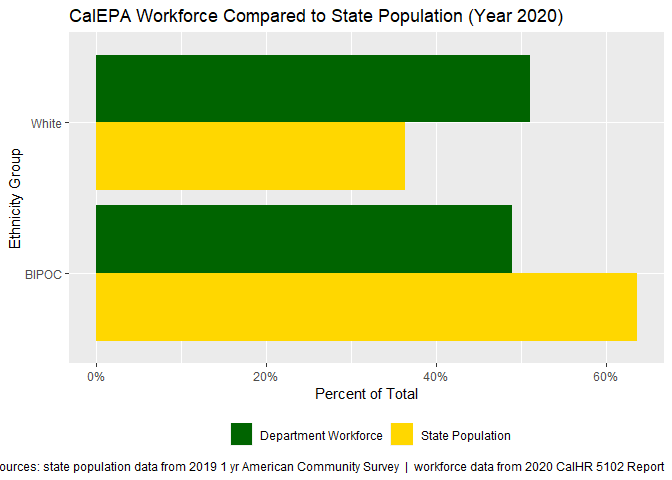
\includegraphics{workforce_metrics_5102_files/figure-latex/unnamed-chunk-8-1.pdf}

\begin{Shaded}
\begin{Highlighting}[]
\NormalTok{(pl\_5102\_dept\_l1\_stack }\OtherTok{\textless{}{-}}\NormalTok{ df\_5102\_dept\_1yr }\SpecialCharTok{\%\textgreater{}\%} 
        \FunctionTok{fun\_summary\_5102\_l1}\NormalTok{() }\SpecialCharTok{\%\textgreater{}\%} 
        \FunctionTok{bind\_rows}\NormalTok{(acs\_data\_level1) }\SpecialCharTok{\%\textgreater{}\%} 
        \FunctionTok{fun\_plot\_5102\_l1\_stack}\NormalTok{(}\AttributeTok{plot\_title =}\NormalTok{ default\_pl\_title, }
                               \AttributeTok{plot\_caption =}\NormalTok{ default\_pl\_caption))}
\end{Highlighting}
\end{Shaded}

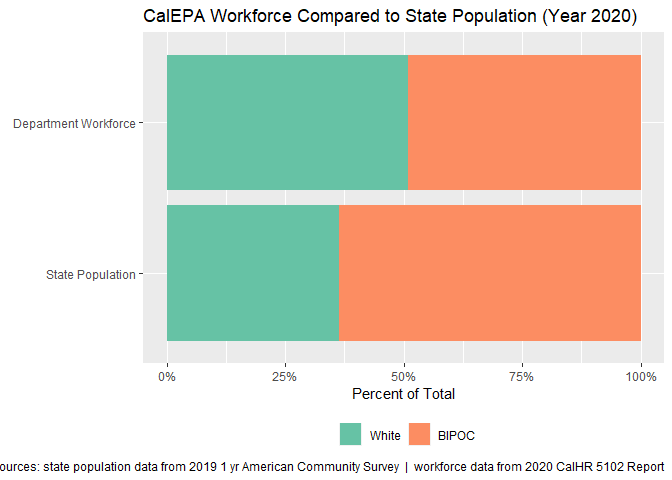
\includegraphics{workforce_metrics_5102_files/figure-latex/unnamed-chunk-8-2.pdf}

\begin{Shaded}
\begin{Highlighting}[]
\CommentTok{\# ggsave(filename = here(\textquotesingle{}07\_slides\textquotesingle{}, \textquotesingle{}2021{-}05{-}14\textquotesingle{}, \textquotesingle{}images\textquotesingle{}, }
\CommentTok{\#                        \textquotesingle{}5102\_dept\_level1\_stack.png\textquotesingle{}), }
\CommentTok{\#        plot = pl\_5102\_dept\_l1\_stack, }
\CommentTok{\#        width = 10, }
\CommentTok{\#        height = 6, }
\CommentTok{\#        dpi = 125}
\CommentTok{\#        )}

\CommentTok{\# \# patchwork (combine plots) {-} Level 1}
\CommentTok{\# pl\_5512\_patch\_dept\_l1 \textless{}{-} pl\_5102\_dept\_l1\_stack / pl\_5102\_dept\_l1}
\end{Highlighting}
\end{Shaded}

\begin{Shaded}
\begin{Highlighting}[]
\DocumentationTok{\#\#\# Level 2 {-}{-}{-}{-}}
\NormalTok{(pl\_5102\_dept\_l2 }\OtherTok{\textless{}{-}}\NormalTok{ df\_5102\_dept\_1yr }\SpecialCharTok{\%\textgreater{}\%} 
     \FunctionTok{fun\_summary\_5102\_l2}\NormalTok{() }\SpecialCharTok{\%\textgreater{}\%} 
     \FunctionTok{bind\_rows}\NormalTok{(acs\_data\_level2) }\SpecialCharTok{\%\textgreater{}\%} 
     \FunctionTok{fun\_plot\_5102\_l2}\NormalTok{(}\AttributeTok{plot\_title =}\NormalTok{ default\_pl\_title, }
                      \AttributeTok{plot\_caption =}\NormalTok{ default\_pl\_caption))}
\end{Highlighting}
\end{Shaded}

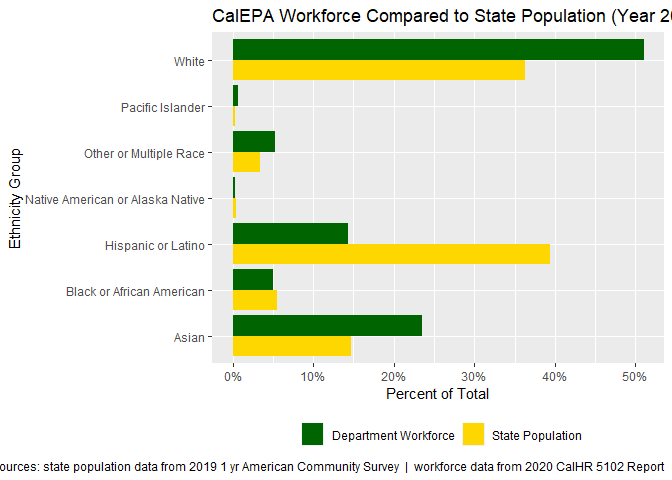
\includegraphics{workforce_metrics_5102_files/figure-latex/unnamed-chunk-9-1.pdf}

\begin{Shaded}
\begin{Highlighting}[]
\CommentTok{\# ggsave(filename = here(\textquotesingle{}07\_slides\textquotesingle{}, \textquotesingle{}2021{-}05{-}14\textquotesingle{}, \textquotesingle{}images\textquotesingle{}, }
\CommentTok{\#                        \textquotesingle{}5102\_dept\_level2.png\textquotesingle{}), }
\CommentTok{\#        plot = pl\_5102\_dept\_l2, }
\CommentTok{\#        width = 10, }
\CommentTok{\#        height = 6, }
\CommentTok{\#        dpi = 125}
\CommentTok{\#        )}

\NormalTok{(pl\_5102\_dept\_l2\_stack }\OtherTok{\textless{}{-}}\NormalTok{ df\_5102\_dept\_1yr }\SpecialCharTok{\%\textgreater{}\%} 
        \FunctionTok{fun\_summary\_5102\_l2}\NormalTok{() }\SpecialCharTok{\%\textgreater{}\%} 
        \FunctionTok{bind\_rows}\NormalTok{(acs\_data\_level2) }\SpecialCharTok{\%\textgreater{}\%} 
        \FunctionTok{fun\_plot\_5102\_l2\_stack}\NormalTok{(}\AttributeTok{plot\_title =}\NormalTok{ default\_pl\_title, }
                               \AttributeTok{plot\_caption =}\NormalTok{ default\_pl\_caption))}
\end{Highlighting}
\end{Shaded}

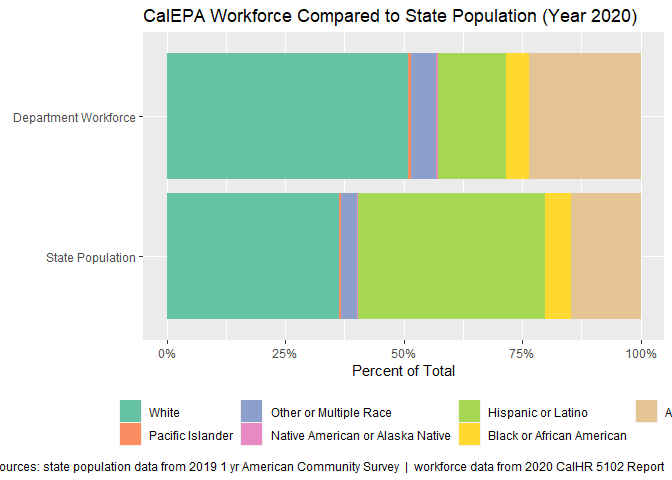
\includegraphics{workforce_metrics_5102_files/figure-latex/unnamed-chunk-9-2.pdf}

\begin{Shaded}
\begin{Highlighting}[]
\CommentTok{\# ggsave(filename = here(\textquotesingle{}07\_slides\textquotesingle{}, \textquotesingle{}2021{-}05{-}14\textquotesingle{}, \textquotesingle{}images\textquotesingle{}, }
\CommentTok{\#                        \textquotesingle{}5102\_dept\_level2\_stack.png\textquotesingle{}), }
\CommentTok{\#        plot = pl\_5102\_dept\_l2\_stack, }
\CommentTok{\#        width = 10, }
\CommentTok{\#        height = 6, }
\CommentTok{\#        dpi = 125}
\CommentTok{\#        )}

\CommentTok{\# patchwork (combine plots) {-} Level 1 and Level 2 stacked plots}
\NormalTok{pl\_5102\_patch\_dept\_stack\_combined }\OtherTok{\textless{}{-}}\NormalTok{ pl\_5102\_dept\_l1\_stack }\SpecialCharTok{/}\NormalTok{ pl\_5102\_dept\_l2\_stack}
\NormalTok{pl\_5102\_patch\_dept\_stack\_combined[[}\DecValTok{1}\NormalTok{]] }\OtherTok{\textless{}{-}}\NormalTok{ pl\_5102\_patch\_dept\_stack\_combined[[}\DecValTok{1}\NormalTok{]] }\SpecialCharTok{+} 
    \FunctionTok{labs}\NormalTok{(}\AttributeTok{title =} \FunctionTok{element\_blank}\NormalTok{(),}
         \AttributeTok{subtitle =} \FunctionTok{element\_blank}\NormalTok{(),}
         \AttributeTok{caption =} \FunctionTok{element\_blank}\NormalTok{())}
\NormalTok{pl\_5102\_patch\_dept\_stack\_combined[[}\DecValTok{2}\NormalTok{]] }\OtherTok{\textless{}{-}}\NormalTok{ pl\_5102\_patch\_dept\_stack\_combined[[}\DecValTok{2}\NormalTok{]] }\SpecialCharTok{+} 
    \FunctionTok{labs}\NormalTok{(}\AttributeTok{title =} \FunctionTok{element\_blank}\NormalTok{(),}
         \AttributeTok{subtitle =} \FunctionTok{element\_blank}\NormalTok{(),}
         \AttributeTok{caption =} \FunctionTok{element\_blank}\NormalTok{())}
\NormalTok{pl\_5102\_patch\_dept\_stack\_combined }\OtherTok{\textless{}{-}}\NormalTok{ pl\_5102\_patch\_dept\_stack\_combined }\SpecialCharTok{+} 
    \FunctionTok{plot\_layout}\NormalTok{(}\AttributeTok{heights =} \FunctionTok{c}\NormalTok{(}\FloatTok{1.7}\NormalTok{, }\DecValTok{2}\NormalTok{)) }\SpecialCharTok{+}
    \FunctionTok{plot\_annotation}\NormalTok{(}
        \AttributeTok{title =}\NormalTok{ default\_pl\_title,}
        \AttributeTok{caption =}\NormalTok{ default\_pl\_caption)}
\CommentTok{\# ggsave(filename = here(\textquotesingle{}07\_slides\textquotesingle{}, \textquotesingle{}2021{-}05{-}14\textquotesingle{}, \textquotesingle{}images\textquotesingle{}, }
\CommentTok{\#                        \textquotesingle{}5102\_dept\_level1\_2\_combined\_stack.png\textquotesingle{}), }
\CommentTok{\#        plot = pl\_5102\_patch\_dept\_stack\_combined, }
\CommentTok{\#        width = 10, }
\CommentTok{\#        height = 6, }
\CommentTok{\#        dpi = 125}
\CommentTok{\#        )}

\CommentTok{\# patchwork (combine plots) {-} both L2 plots}
\NormalTok{pl\_5102\_patch\_dept\_l2 }\OtherTok{\textless{}{-}}\NormalTok{ pl\_5102\_dept\_l2\_stack }\SpecialCharTok{/}\NormalTok{ pl\_5102\_dept\_l2}
\NormalTok{pl\_5102\_patch\_dept\_l2[[}\DecValTok{1}\NormalTok{]] }\OtherTok{\textless{}{-}}\NormalTok{ pl\_5102\_patch\_dept\_l2[[}\DecValTok{1}\NormalTok{]] }\SpecialCharTok{+} 
    \FunctionTok{labs}\NormalTok{(}\AttributeTok{title =} \FunctionTok{element\_blank}\NormalTok{(),}
         \AttributeTok{subtitle =} \FunctionTok{element\_blank}\NormalTok{(),}
         \AttributeTok{caption =} \FunctionTok{element\_blank}\NormalTok{())}
\NormalTok{pl\_5102\_patch\_dept\_l2[[}\DecValTok{2}\NormalTok{]] }\OtherTok{\textless{}{-}}\NormalTok{ pl\_5102\_patch\_dept\_l2[[}\DecValTok{2}\NormalTok{]] }\SpecialCharTok{+} 
    \FunctionTok{labs}\NormalTok{(}\AttributeTok{title =} \FunctionTok{element\_blank}\NormalTok{(),}
         \AttributeTok{subtitle =} \FunctionTok{element\_blank}\NormalTok{(),}
         \AttributeTok{caption =} \FunctionTok{element\_blank}\NormalTok{())}
\NormalTok{pl\_5102\_patch\_dept\_l2 }\OtherTok{\textless{}{-}}\NormalTok{ pl\_5102\_patch\_dept\_l2 }\SpecialCharTok{+} 
    \FunctionTok{plot\_annotation}\NormalTok{(}
        \AttributeTok{title =}\NormalTok{ default\_pl\_title,}
        \AttributeTok{caption =}\NormalTok{ default\_pl\_caption)}
\CommentTok{\# ggsave(filename = here(\textquotesingle{}07\_slides\textquotesingle{}, \textquotesingle{}2021{-}05{-}14\textquotesingle{}, \textquotesingle{}images\textquotesingle{}, }
\CommentTok{\#                        \textquotesingle{}5102\_dept\_level2\_combined.png\textquotesingle{}), }
\CommentTok{\#        plot = pl\_5102\_patch\_dept\_l2, }
\CommentTok{\#        width = 10, }
\CommentTok{\#        height = 6, }
\CommentTok{\#        dpi = 125}
\CommentTok{\#        )}
\end{Highlighting}
\end{Shaded}


\end{document}
